\subsection*{Applicazione della teoria di Dyson}
Si parte da una Hamiltoniana $\H_0$, a cui si aggiunge una perturbazione dipendente dal tempo $V(t)$. Nella rappresentazione di Interazione lo stato è
\[
	\Ket{\psi(t)} = \U(t)\Ket {\psi(0)} = e^{\frac{i}{\hslash} \H_0 t} \Ket{\psi(0)} = e^{-\frac{i}{\hslash} \H_0 t} \Ket{\psi_I(t)}
\]
e le proiezioni sugli autostati di $\H(t)$ dipendono dal tempo:
\begin{gather*}
	C_n(t) = \braket{n} {\psi(t)} = e^{-\frac{i}{\hslash} \H_0 t} \braket{n} {\psi_I(t)} = \\
	= e^{-\frac{i}{\hslash} E_n t} \Bra{n} \left[ \Ket{\psi_I(0)} + \cdots (\text{sviluppo di Dyson}) \right]
\end{gather*}
In questa espansione possiamo introdurre direttamente il termine $\Bra n$ per aver un risultato più specifico, inoltre dichiariamo $\Ket {\psi{(0)}} = \Ket {\psi_I(0)} = \Ket m$ e $n \neq m$:
\[
	C_n(t) = e^{-\frac{i}{\hslash} E_n t} \left[ \cancel{\braket{n}{m}} + \frac{1}{i\h} \tint \braketin{n}{\V_I(t')}{m} dt' + (\frac{1}{i\h})^2 \tint \tint[t'] \braketin{n}{\V_I(t')\V_I(t'')}{m} dt'' dt' + \cdots \right]
\]
ora, ricordando la definizione di operatore in rappresentazione d'interazione possiamo espandere in maniera più comoda gli integrali:
\[
	\tint \braketin{n}{\V_I(t')}{m} dt' = \tint \braketin{n}{e^{\frac{i}{\hslash} \H_0 t}\V(t') e^{-\frac{i}{\hslash} \H_0 t'}}{m} dt' = \tint e^{\frac{i}{\hslash} \omega_{nm} t'} \braketin{n}{\V(t')}{m} dt'
\]
dove $\omega_{nm} = E_m - E_n$ è la differenza tra le energie dei livelli $m$ e $n$. E similmente si ottiene (inserendo una completezza tra i due $\V_I$):
\[
	\tint \tint[t'] \braketin{n}{\V_I(t')\V_I(t'')}{m} dt'' dt' = \sum_{k} \tint e^{\frac{i}{\hslash} \omega_{nk} t'} \tint[t'] e^{\frac{i}{\hslash} \omega_{km} t''} \braketin{n}{\V(t')\V(t'')}{m} dt'' dt'
\]

All'atto pratico quello che queste espressioni calcolano non è altro che una misura di "quanto la perturbazione tende a far saltare tra gli stati". Il primo ordine misura solo i salti diretti, il secondo ordine misura tutti i salti con due passaggi, e così via! Sommando tutto si ha la probabilità che in un qualsiasi modo lo stato $\Ket m$ sia passato allo stato $\Ket n$ a causa della perturbazione.
\subsection*{Esercizio: potenziale costante}
Si consideri una perturbazione costante nel tempo $V(t) = V$ per $t \geq 0$ e nulla per $t < 0$. Chiamiamo $f$ una funzione step che rente continua la discontinuità in $t=0$, per cui $V(t) = V f(t)$. \\
La probabilità di passare da uno stato $i$ a uno stato $n$, al primo ordine, è
\[
	P_{i \to n}(t) = \frac{1}{\hslash^2} \left| \int_0^t \Bra{n} V_I(t') \Ket{i} dt' \right|^2 = \frac{1}{\hslash^2} \left| V_{n,i} \int_0^t e^{i \omega_{n,i} t'} dt' \right|^2 = \]\[
	= \frac{|V_{n,i}|^2}{\hslash^2} \left| \frac{e^{i \omega_{n,i} t} - 1}{i \omega_{n,i}} \right|^2 = \frac{4 |V_{n,i}|^2}{\hslash^2 \omega_{n,i}^2} \sin^2 \left( \frac{\omega_{n,i} t}{2} \right)
\]

% Inserire nel preambolo: 
\begin{center}
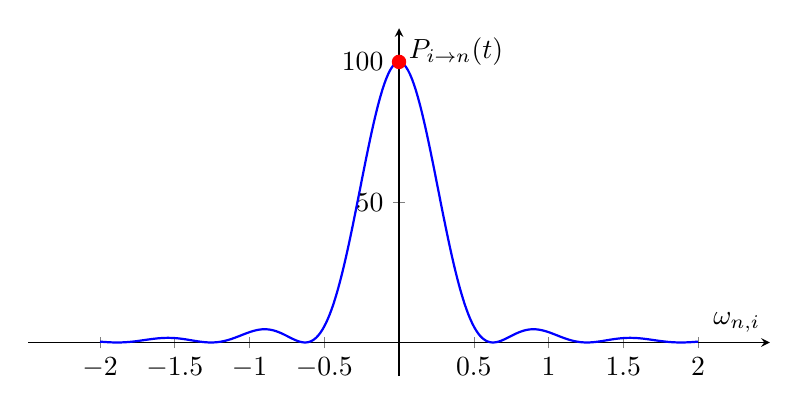
\begin{tikzpicture}
	\def\V{1} % |V_{n,i}|
	\def\hbar{1} % \hslash
	\def\t{10} % tempo t
	\pgfmathsetmacro{\A}{4*(\V)^2/(\hbar)^2}
	\pgfmathsetmacro{\yzero}{(\V)^2*(\t)^2/(\hbar)^2} % limite ω->0
	\begin{axis}[
		domain=-2:2,
		samples=300,
		xlabel={$\omega_{n,i}$},
		ylabel={$P_{i\to n}(t)$},
		axis lines=middle,
		enlargelimits=0.12,
		ymin=0,
		width=11cm,height=6cm,
		legend cell align=left
	]
		% funzione: P(ω) = A * sin^2(ω t /2) / ω^2, usare deg(...) perché pgfmath sin() prende gradi
		\addplot[blue,thick] { \A * ( (sin(deg(x*\t/2)))^2 / (x^2) ) };
		% \addlegendentry{ $P(\omega)=\dfrac{4|V|^2}{\hbar^2}\dfrac{\sin^2(\omega t/2)}{\omega^2}$ }
		% punto al limite ω->0
		\addplot[red,only marks,mark=*,mark options={scale=1.2}] coordinates {(0,\yzero)};
	\end{axis}
\end{tikzpicture}
\end{center}

Risulta che l'area sottesa alla curva cresce linearmente col tempo, mentre la quantità di stati che ha senso prendere in considerazione è inversamente proporzionale ($\Delta E \sim \hslash 4 \pi/t$). Quindi la probabilità di transizione per unità di tempo, all'ordine lineare, tende a una costante.

Quel che risulta in generale è che questa teoria perturbativa è valida alle stesse condizioni della teoria l'altra, ovvero quanto
\[
	\pi|V_{n,i}| \ll |E_n - E_i|
\]

Risalta anche la relazione di incertezza tempo-energia, ovvero $\Delta E \Delta t \sim \hslash$.

\subsection*{Ampiezza di correlazione e Relazione tempo-energia}
Ci si può chiedere, quanto differiscono $\Ket {\psi(t)}$ e $\Ket{\psi(0)}$? Come si confrontano? Si definisce la \textbf{funzione di correlazione}\index{Funzione di correlazione} come
\[
	\Co(t) = \braket{\psi(0)}{\psi(t)} = \Bra{\psi(0)} U(t,0) \ket{\psi(0)}
\]
Essa misura la sovrapposizione tra lo stato iniziale e lo stato evoluto. Chiaramente coincide col valor medio dell'operatore di evoluzione temporale nello stato iniziale:
\[
	\Co(t) = \avg[0]{U(t,0)}
\]

Se in un sistema ortonormale completo si ha uno stato $\Ket \psi = \sum_n C_n\Ket n$, al chè la funzione di correlazione è esprimibile come:
\[
	\Co(t) = \sum_n |C_n|^2 e^{-\frac{i}{\hslash} E_n t}
\]

Supponiamo ora il caso in cui gli stati sono molto densi, quasi continui ma ancora discreti; ha senso a questo punto definire una \textbf{densità di stati}\index{Densità di stati} $\rho(E)$, tale che $\rho(E) dE$ è il numero di stati con energia compresa tra $E$ e $E + dE$. Allora la funzione di correlazione può essere riscritta come
\[
	\Co(t) = \int |C(E)|^2 \rho(E) e^{-\frac{i}{\hslash} E t} dE
\]
dove $|C(E)|^2$ è la probabilità di trovare lo stato con energia $E$. Se ci si restringe a una distribuzione comoda di stati, ad esempio una gaussiana centrata in $E_0$ con varianza $\Delta E$, si ottiene:
\[
	\Co(t) = \int \frac{\rho(E - E_0)}{\sqrt{2 \pi} \Delta E} e^{-\frac{(E - E_0)^2}{2 \Delta E^2}} e^{-\frac{i}{\hslash} E t} dE = \rho(E_0)e^{-\frac{i}{\hslash} E_0 t} e^{-\frac{t^2 \Delta E^2}{2 \hslash^2}}
\]
Tenendo conto del secondo esponenziale, si può dedurre che la funzione di correlazione decade su una scala temporale $\Delta t \sim \frac{\hslash}{\Delta E}$, che è proprio la relazione di incertezza tempo-energia!